\documentclass{beamer}
 
 \usetheme{Madrid}
\usepackage[utf8]{inputenc}
 
 
%Information to be included in the title page:
\title[Early Warning Signals] %optional
{A Novel Scaling Indicator of Early Warning Signals}

\subtitle{with an application to tropical cyclones}

\author[Joshua Prettyman] % (optional, for multiple authors)
{Joshua Prettyman\inst{1,2} \and Tobias Kuna\inst{1} \and Valerie Livina\inst{2}}

\institute[] % (optional)
{
	\inst{1}%
	University of Reading
	\and
	\inst{2}%
	National Physical Laboratory 
}

\date[September2018] % (optional)
{Doctoral Training Showcase in Mathematics of Planet Earth, September 2018

\begin{figure}
	\centering

\includegraphics[height=0.5cm]{figures/logo.png}
 \end{figure}
}
 
 
\begin{document}
 
\frame{\titlepage}
 
\begin{frame}{Early warning signals of tipping points}
\begin{columns}
\begin{column}{0.4\paperwidth}
Tipping point: an abrupt change in a system
\vspace{0.5cm}

We want to predict the tipping point
\vspace{0.5cm}

We can use
\begin{itemize}
	\item Variance 
	\item Autocorrelation
	\item DFA
	\item Potential analysis
	\item Model fitting
\end{itemize}
\end{column}
\pause
\begin{column}{0.4\paperwidth}
	\begin{figure}
		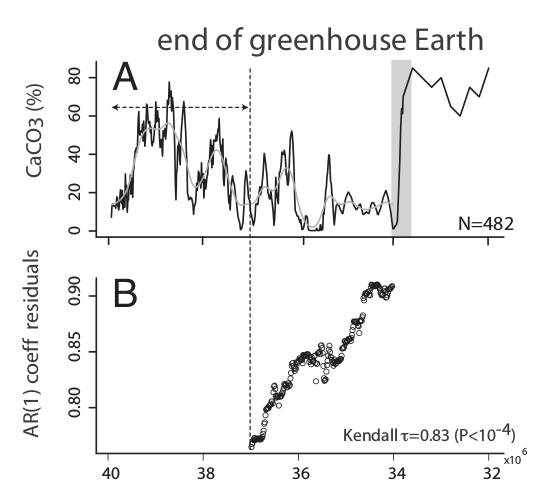
\includegraphics[width=\linewidth]{figures/greenhouse.png}
		\caption{\scriptsize Dakos, V., Scheffer, M., van Nes, E. H., Brovkin, V.,Petoukhov, V. and Held, H. (2008).
			Slowing down as an early warning signal for abrupt climate change. {\it Proc. Nat. Acad. Sci. USA 105, 14308-14312.}}
	\end{figure}

\end{column}
\end{columns}
 \end{frame}

\begin{frame}{The pitchfork bifurcation}
\begin{columns}
	\begin{column}{0.4\paperwidth}
		\begin{equation*}
		\dot{z} = -\frac{\partial}{\partial z}\left(z^4 - \mu_t z^2\right) + \eta_t 
		\end{equation*}
		
		\begin{figure}
			\centering
			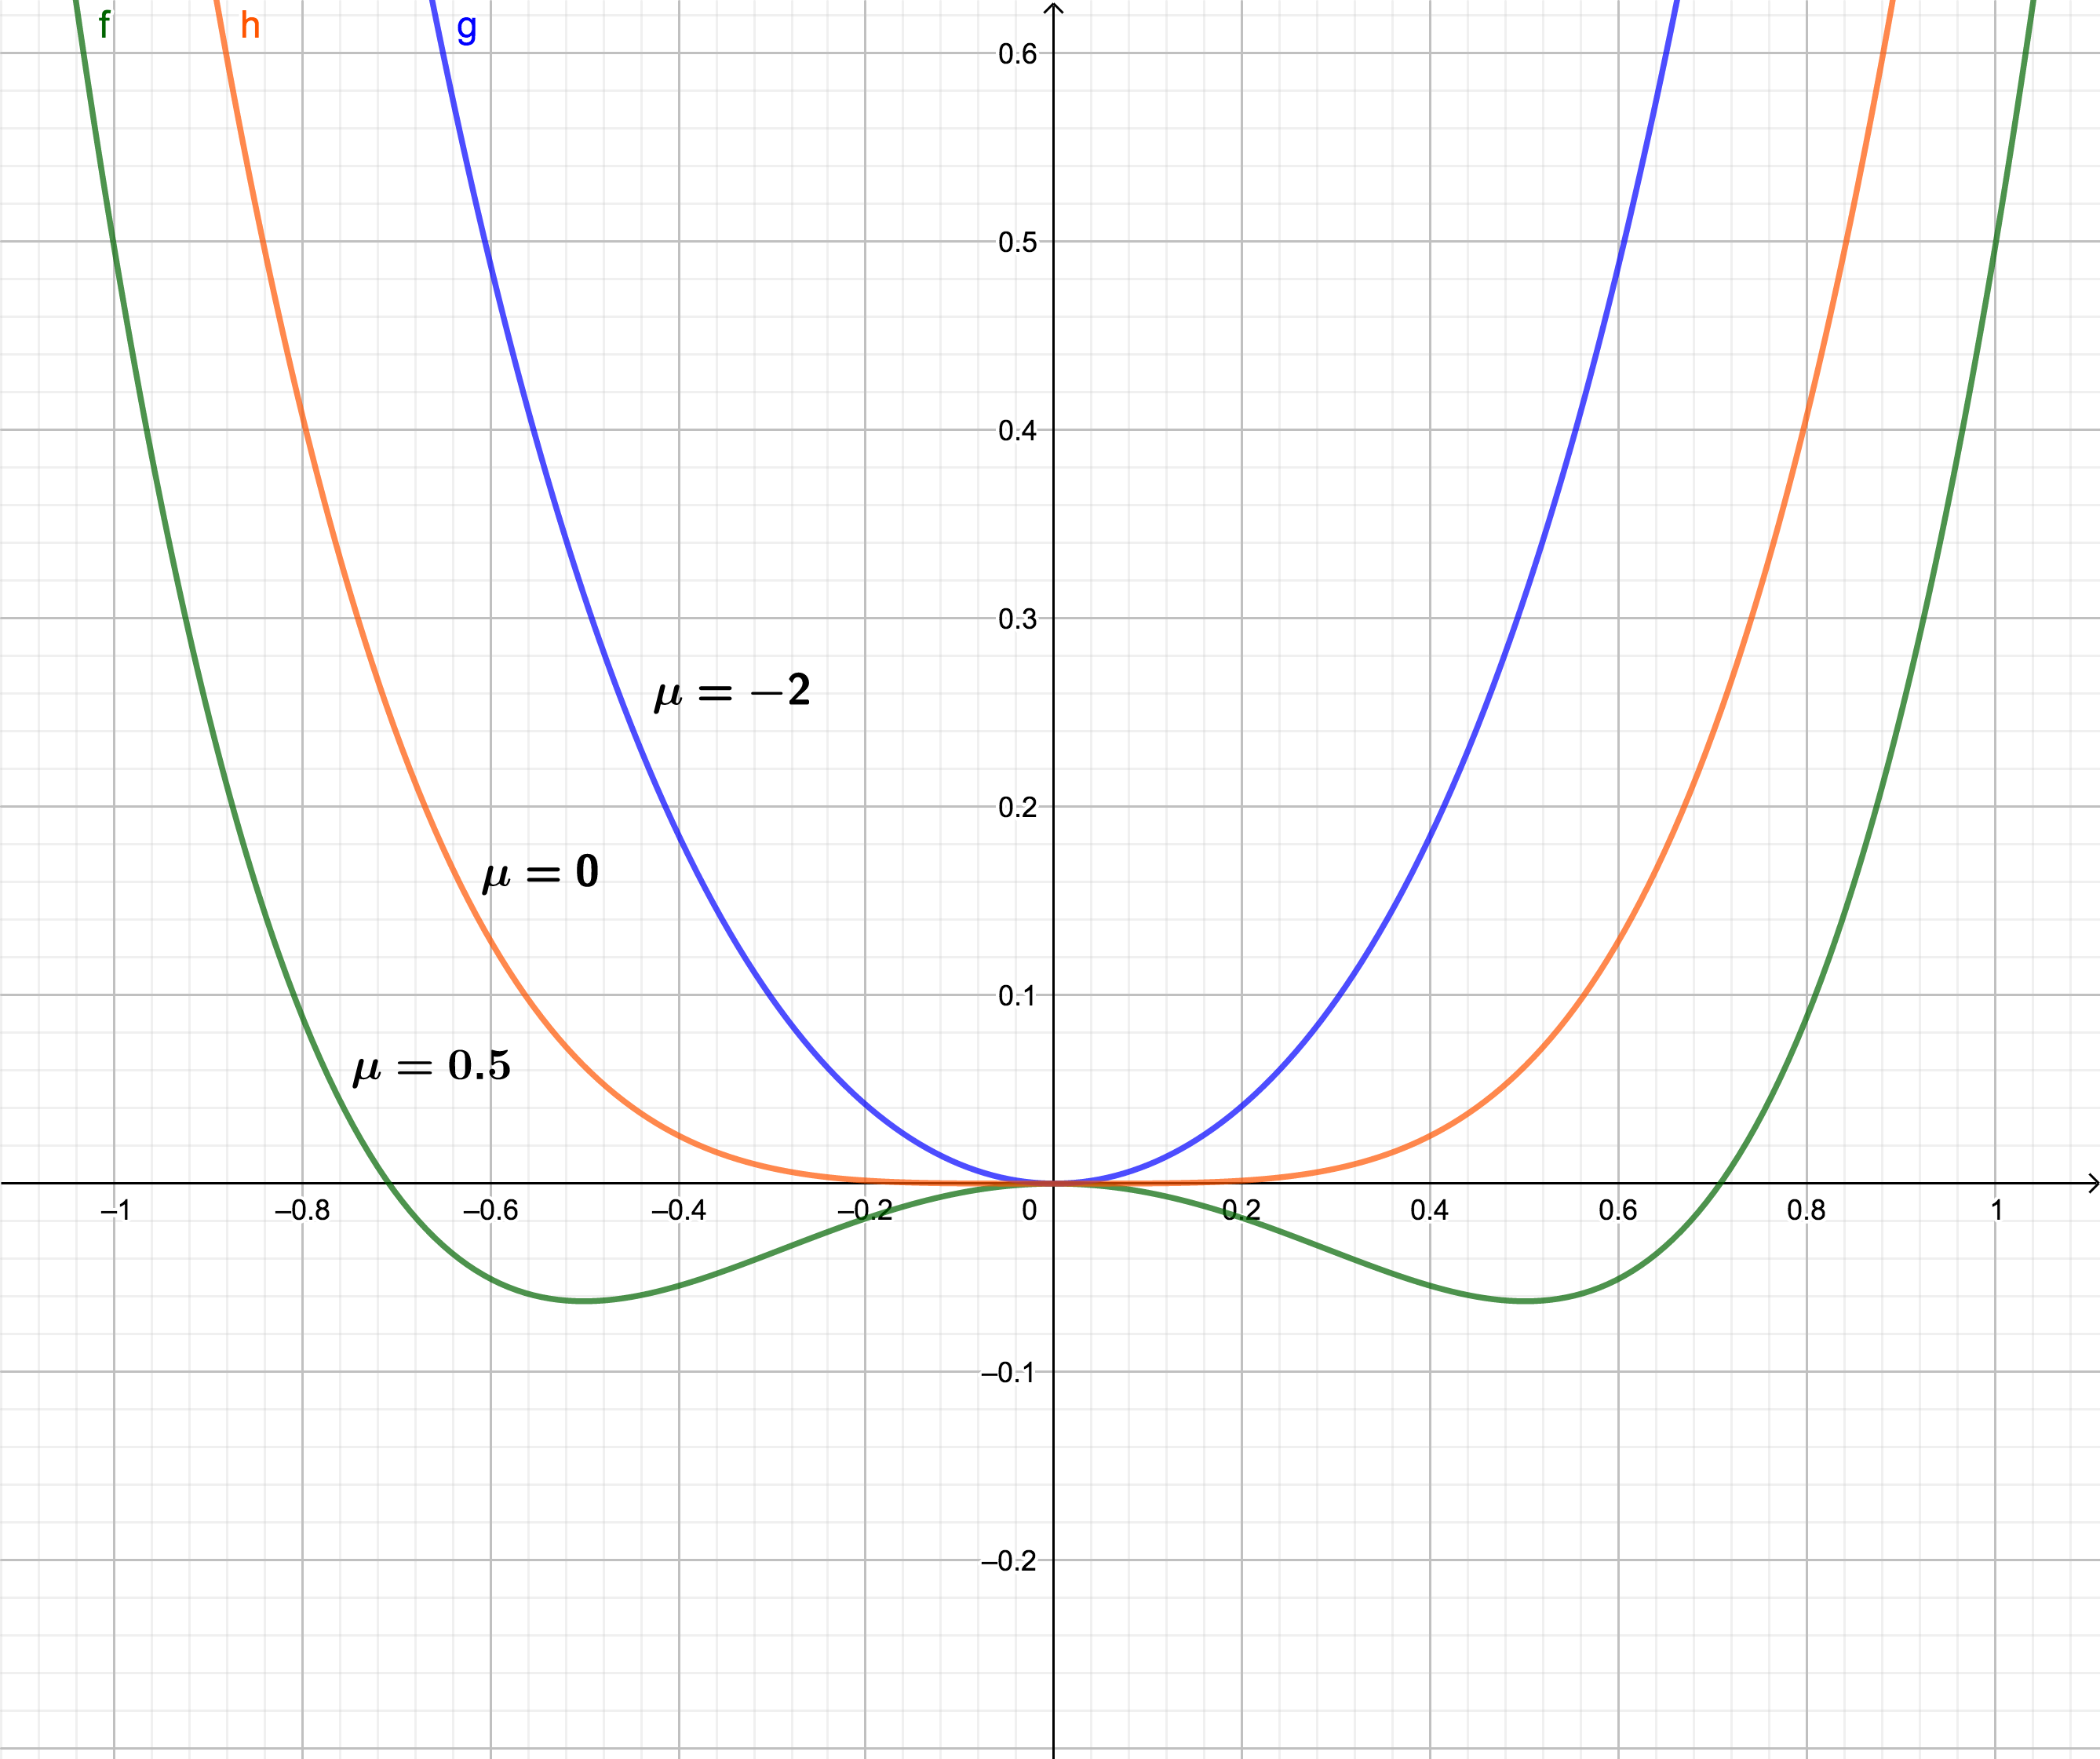
\includegraphics[width=0.8\linewidth]{figures/PitchforkGeogebra.png}
		\end{figure}
	
		\begin{center}
		Bifurcation at $\mu = 0$.
		\end{center}
	\end{column}

	\begin{column}{0.4\paperwidth}
		\begin{figure}
			\centering
			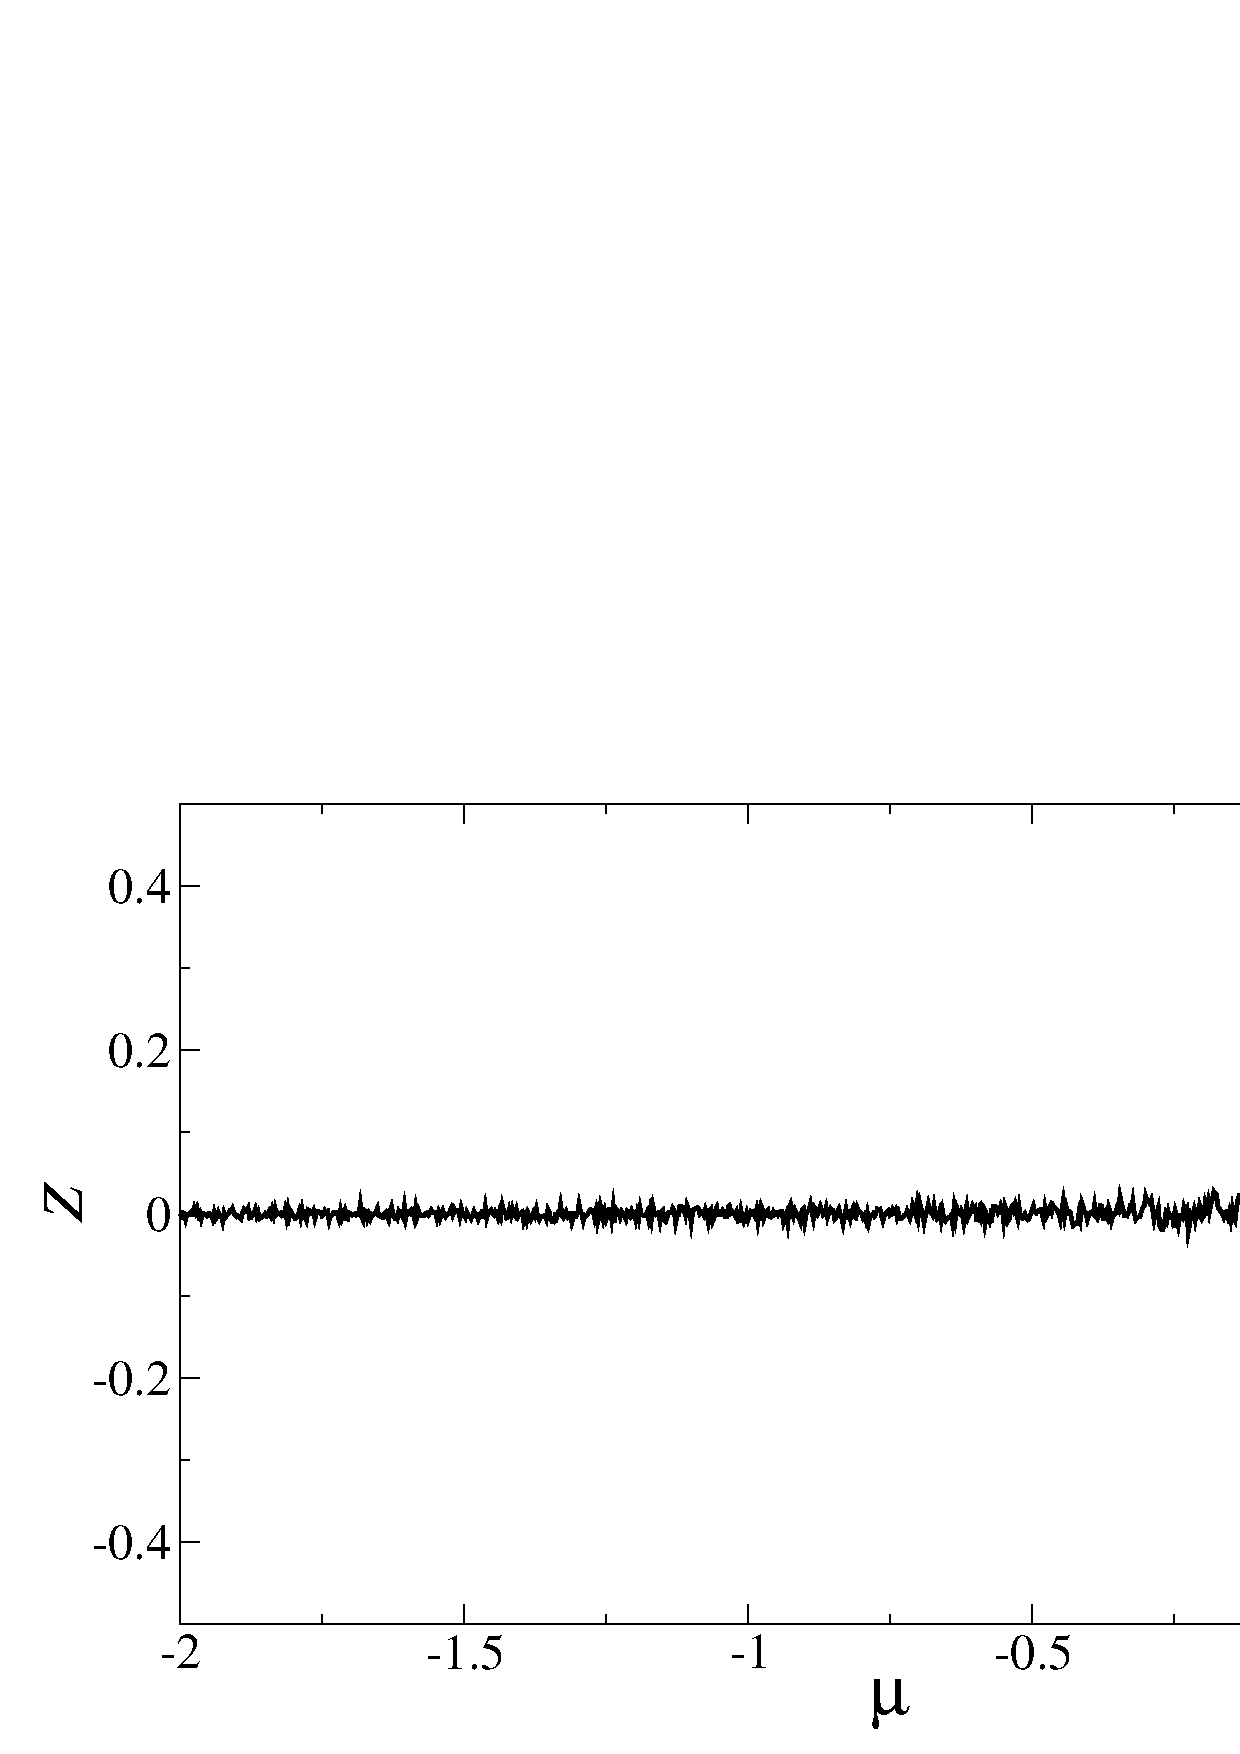
\includegraphics[width=\linewidth]{figures/Z1}
		\end{figure}
		\pause
		\begin{figure}
		\centering
		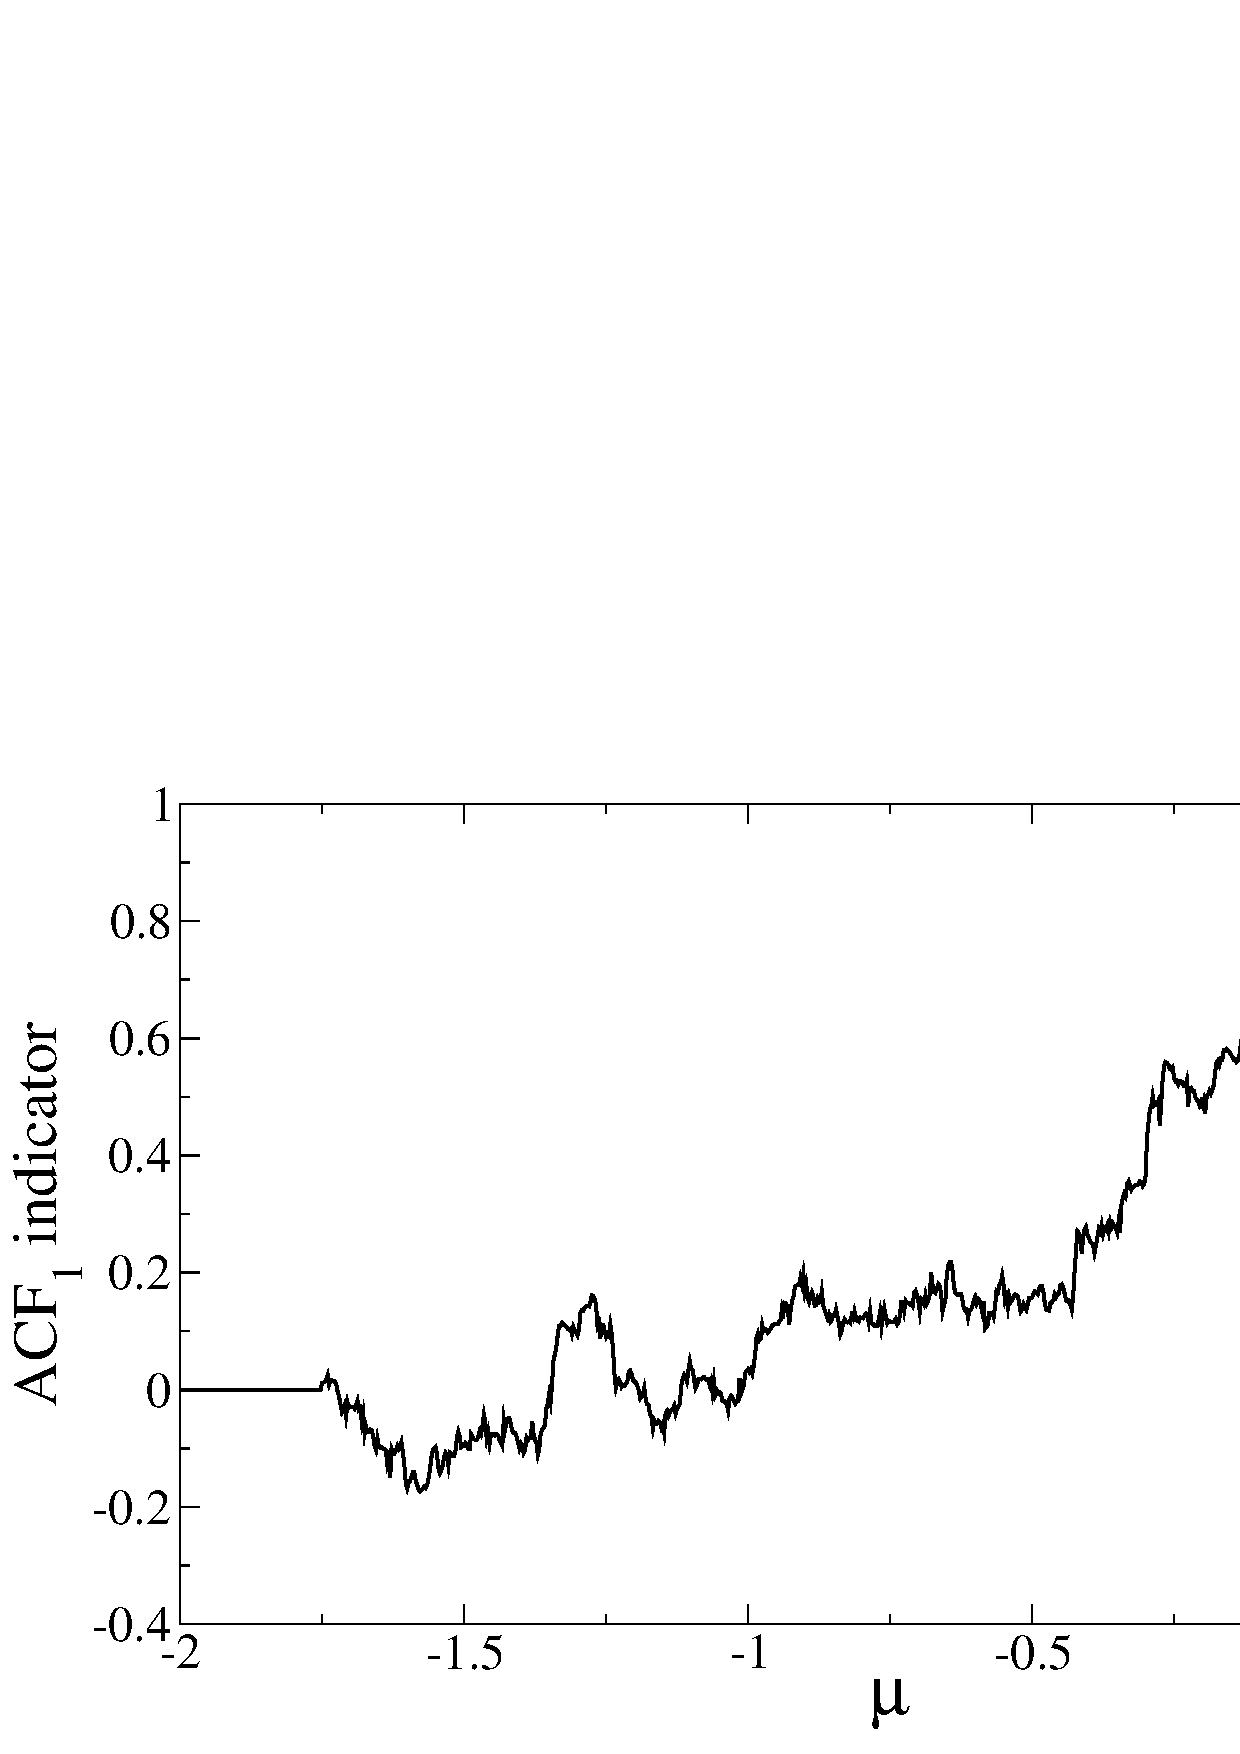
\includegraphics[width=\linewidth]{figures/ACF1}
		\end{figure}
	\end{column}
\end{columns}
\end{frame}


\begin{frame}{The pitchfork bifurcation}
\begin{columns}
	\begin{column}{0.4\paperwidth}
		
		\begin{equation*}
		\dot{z} = -\frac{\partial}{\partial z}\left(z^4 - \mu_t z^2\right) + \eta_t 
		\end{equation*}
		
		\begin{figure}
			\centering
			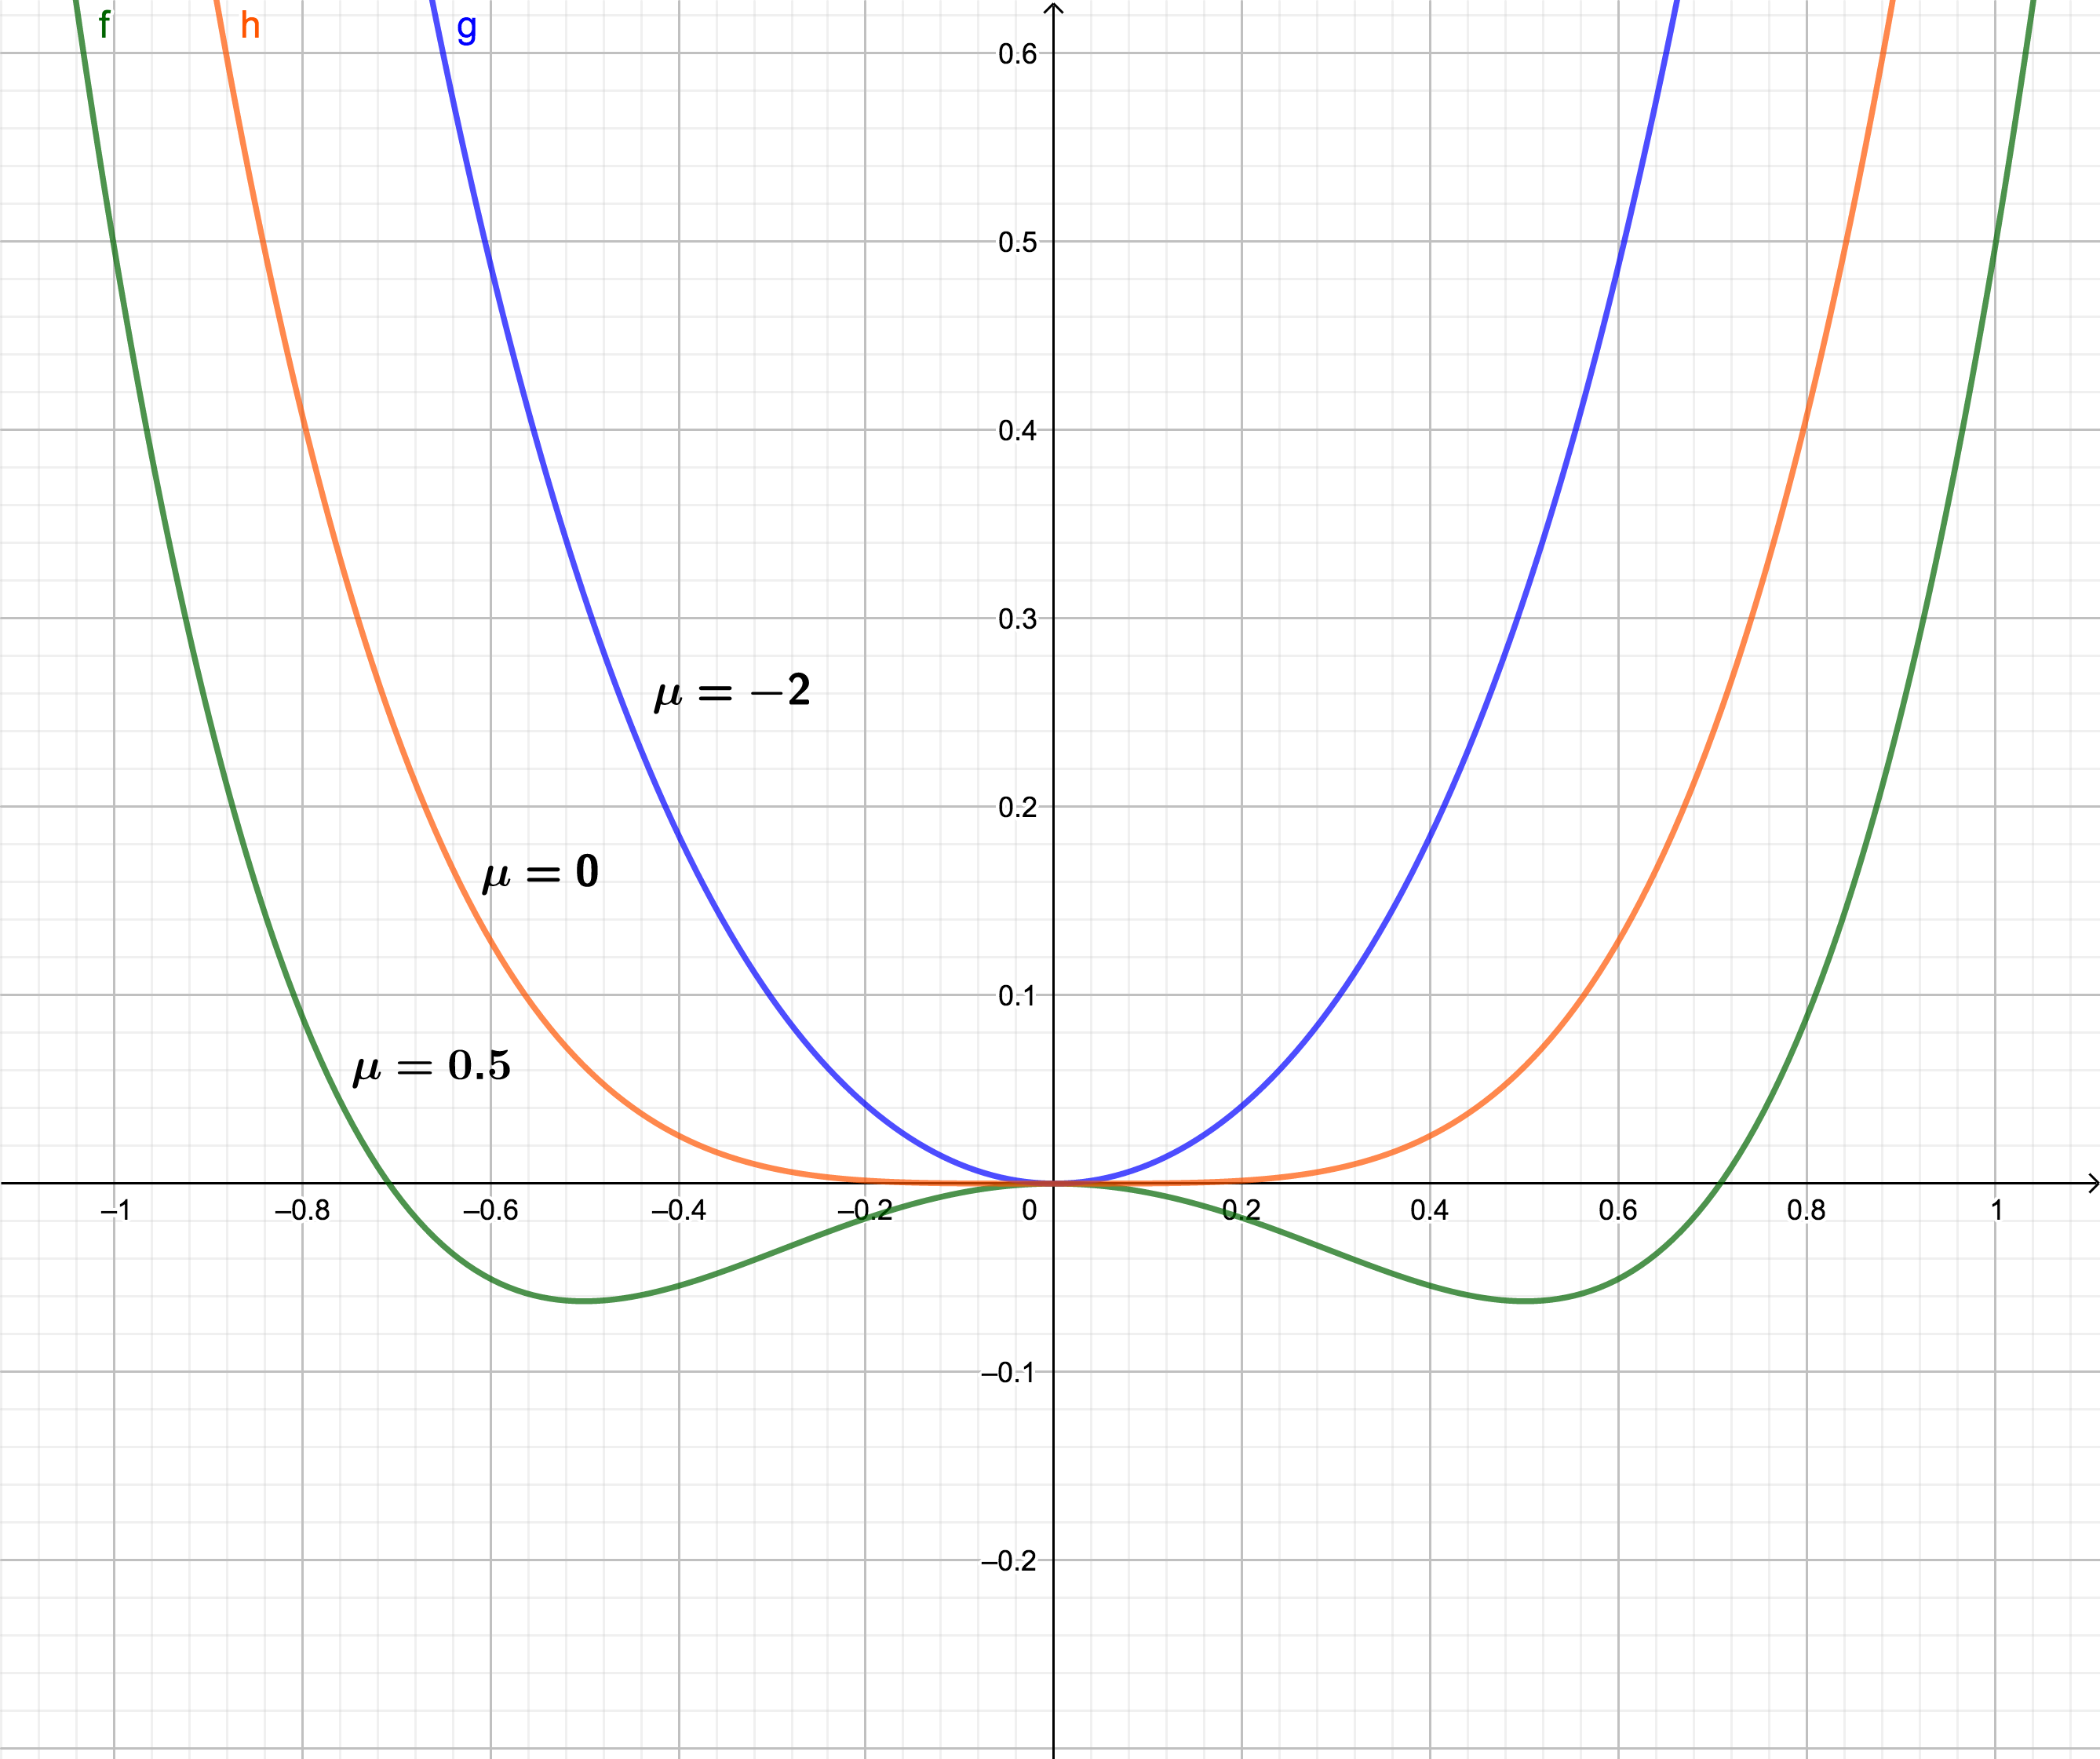
\includegraphics[width=0.8\linewidth]{figures/PitchforkGeogebra.png}
		\end{figure}
		
		\begin{center}
			Bifurcation at $mu = 0$.
		\end{center}
	\end{column}

	\begin{column}{0.4\paperwidth}
		\begin{figure}
			\centering
			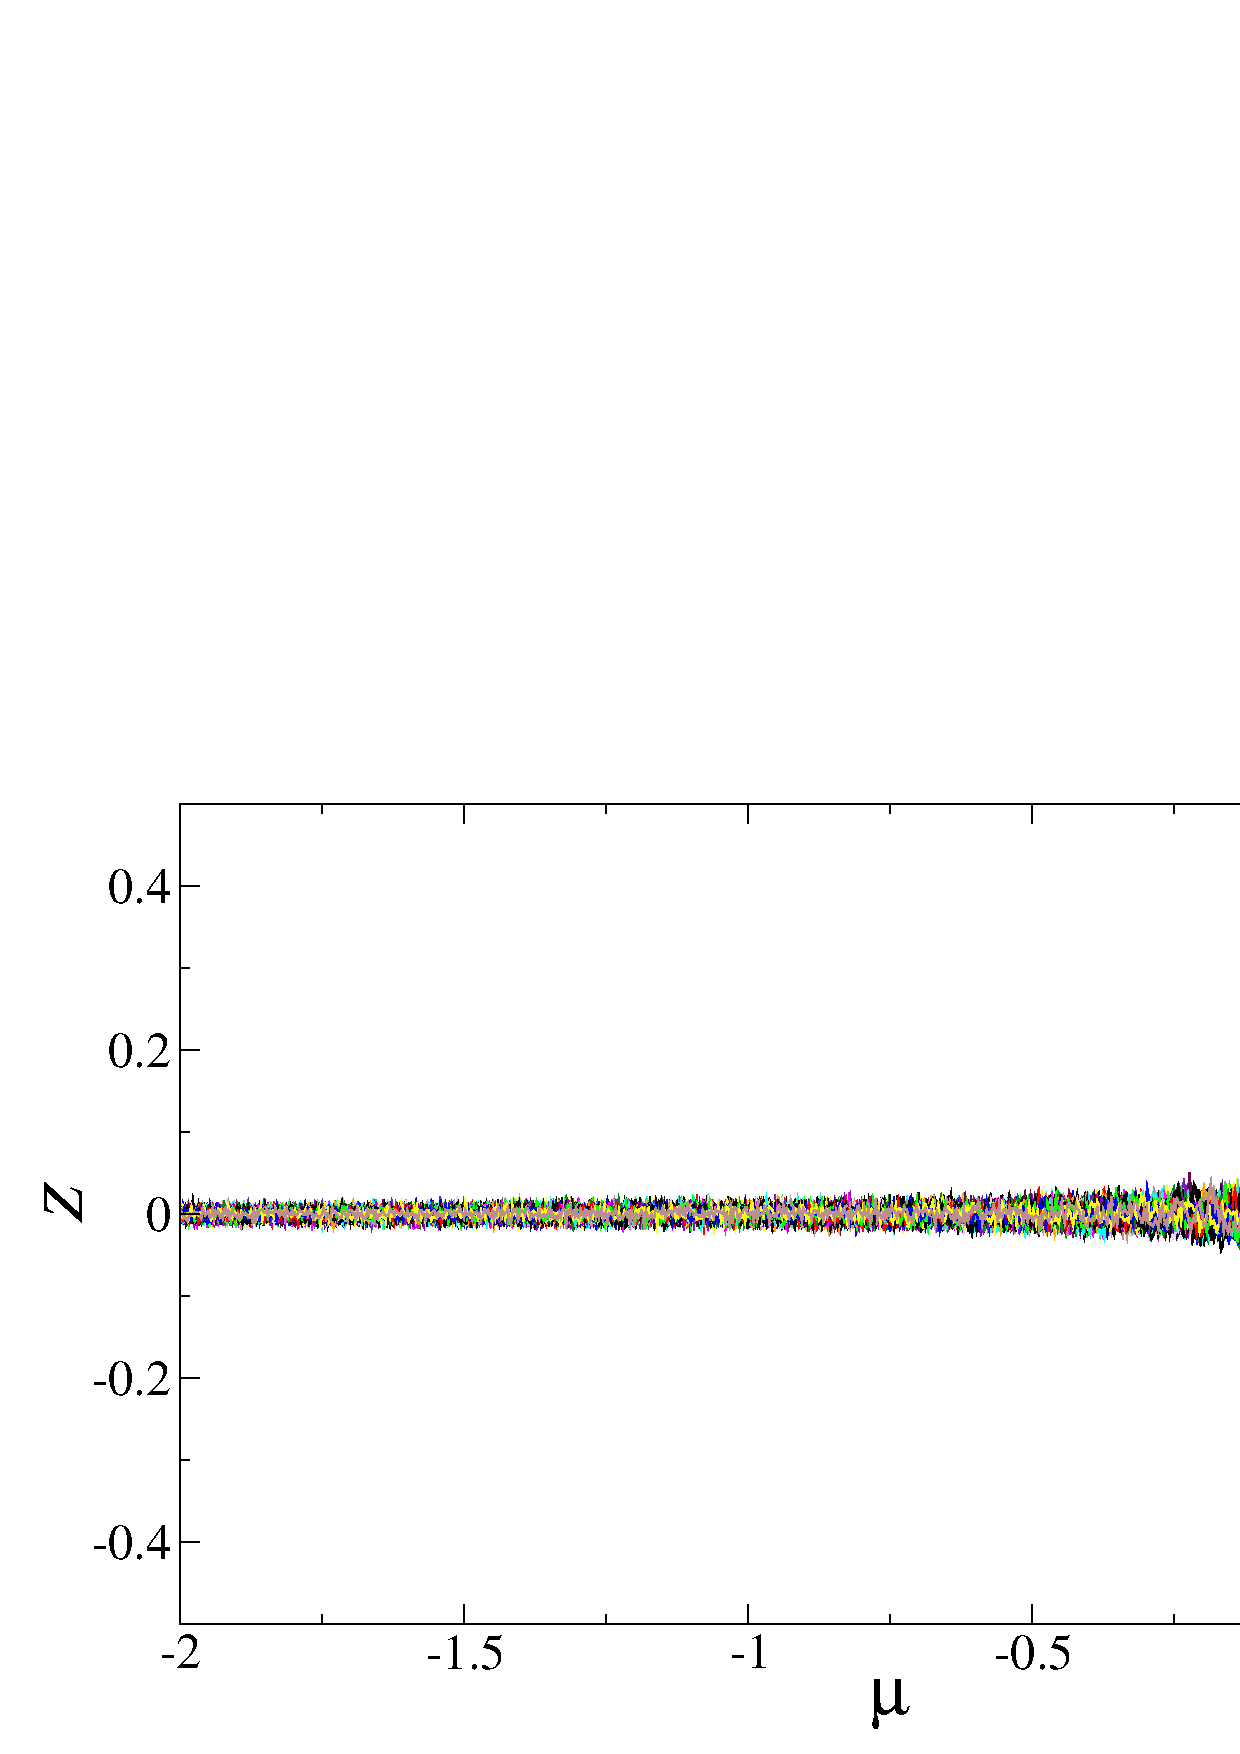
\includegraphics[width=\linewidth]{figures/Z100}
		\end{figure}

		\begin{figure}
			\centering
			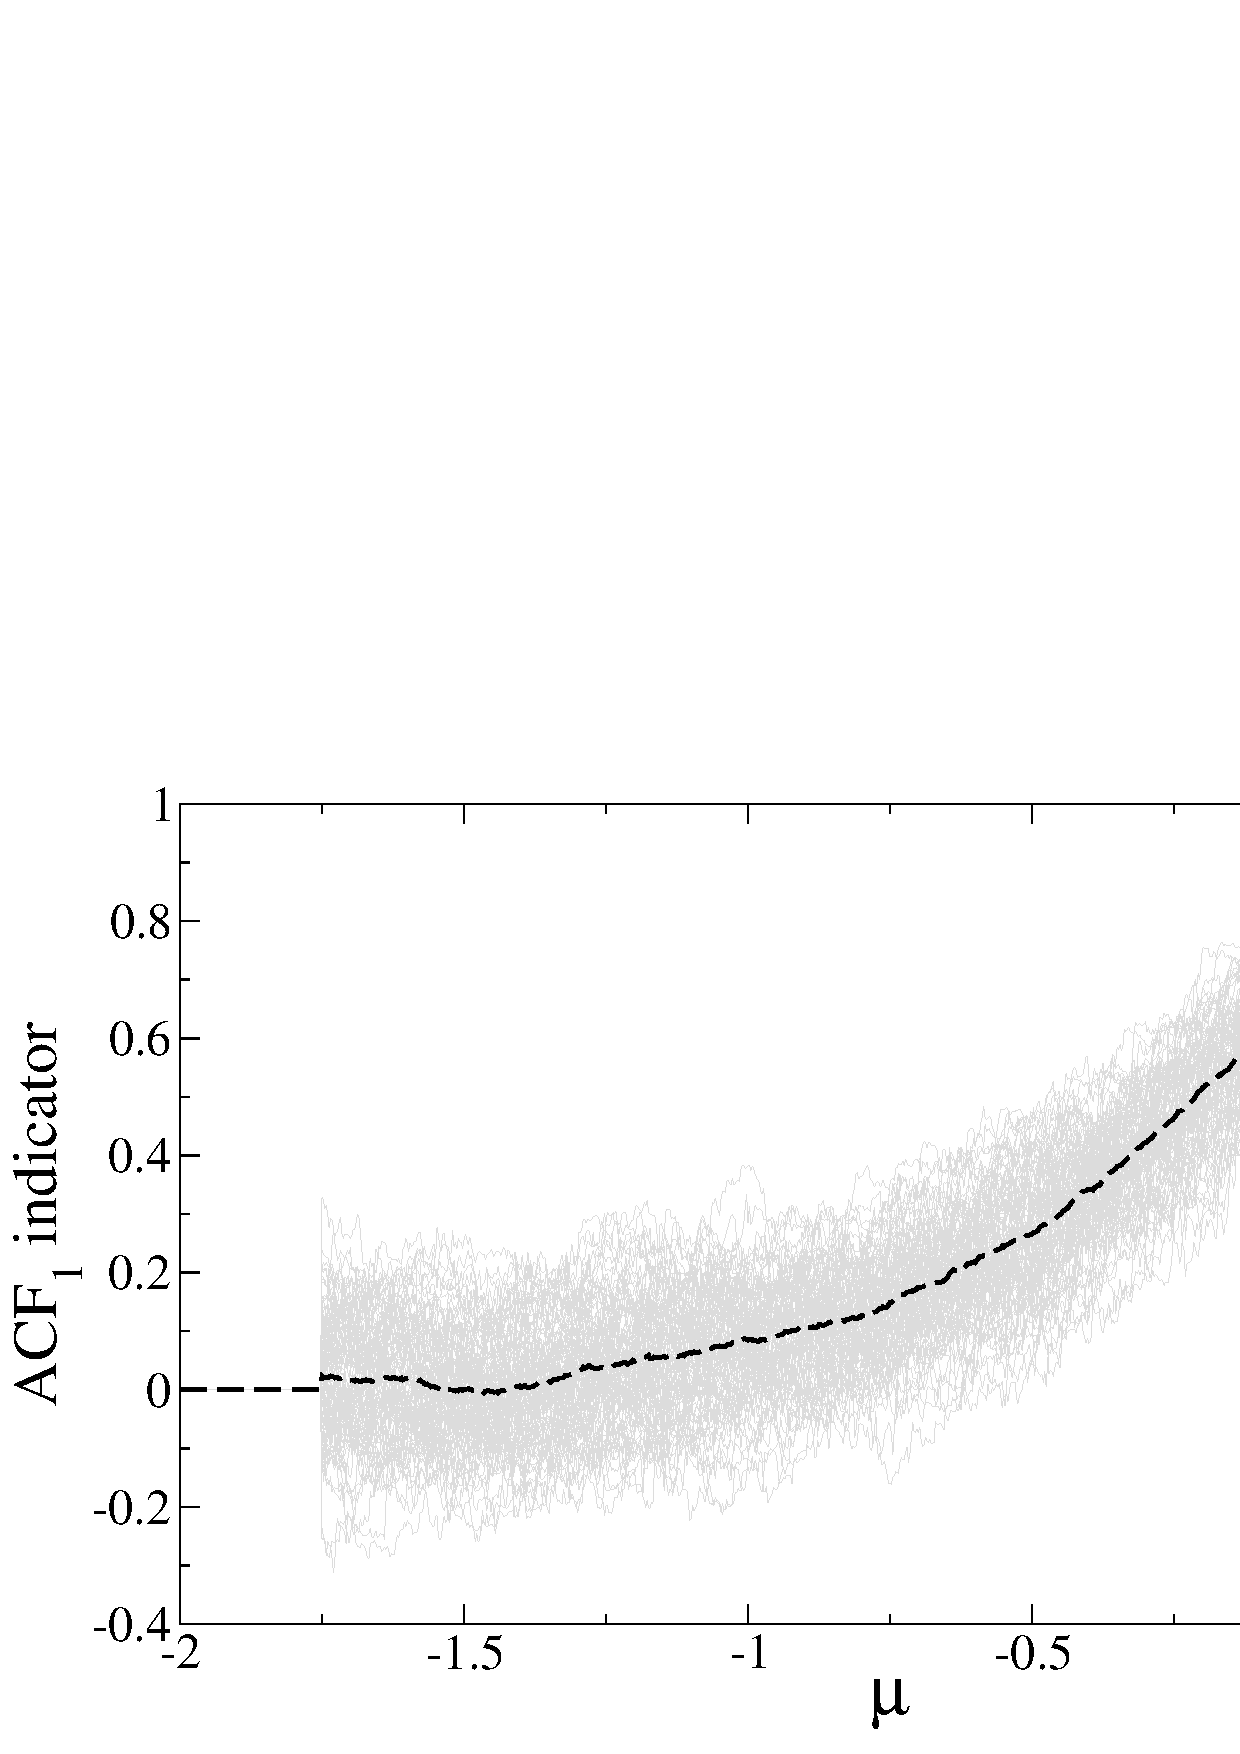
\includegraphics[width=\linewidth]{figures/ACF100}
		\end{figure}
	\end{column}
\end{columns}
\note{It makes sense that as the potential functions gets wider, the series starts to look less like white noise which has ACF=0 and more like brownian motion with ACF=1. 

But if we are talking about white noise and red noise, why use the ACF? Why not use the method that you would normally use to measure the colour of a signal?}

\end{frame}

\begin{frame}{Colours of noise}

\begin{columns}
	\begin{column}{0.4\paperwidth}
		\centering
		White
		
		\begin{figure}
			\centering
			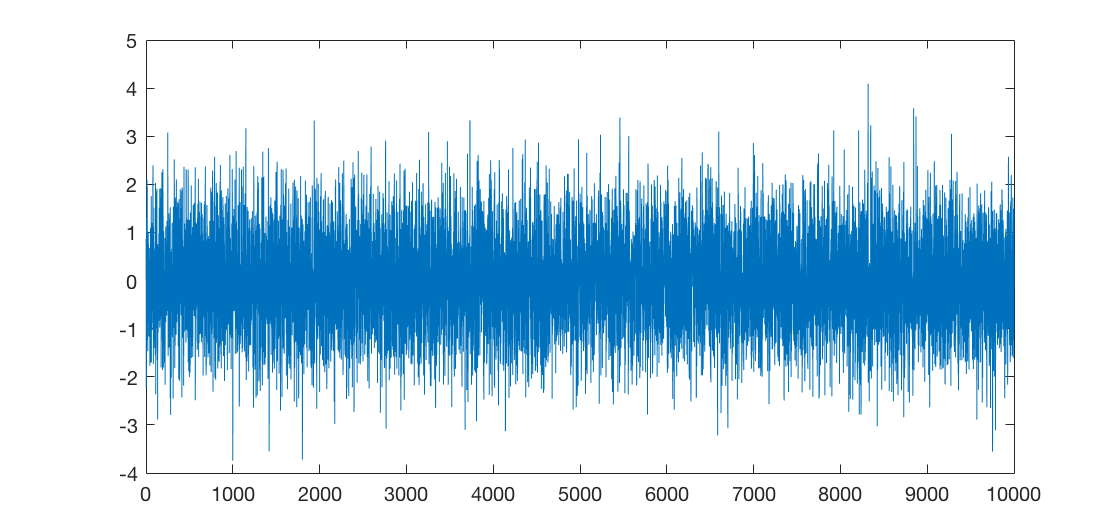
\includegraphics[width=0.8\linewidth]{figures/xw.png}
		\end{figure}
		\begin{figure}
			\centering
			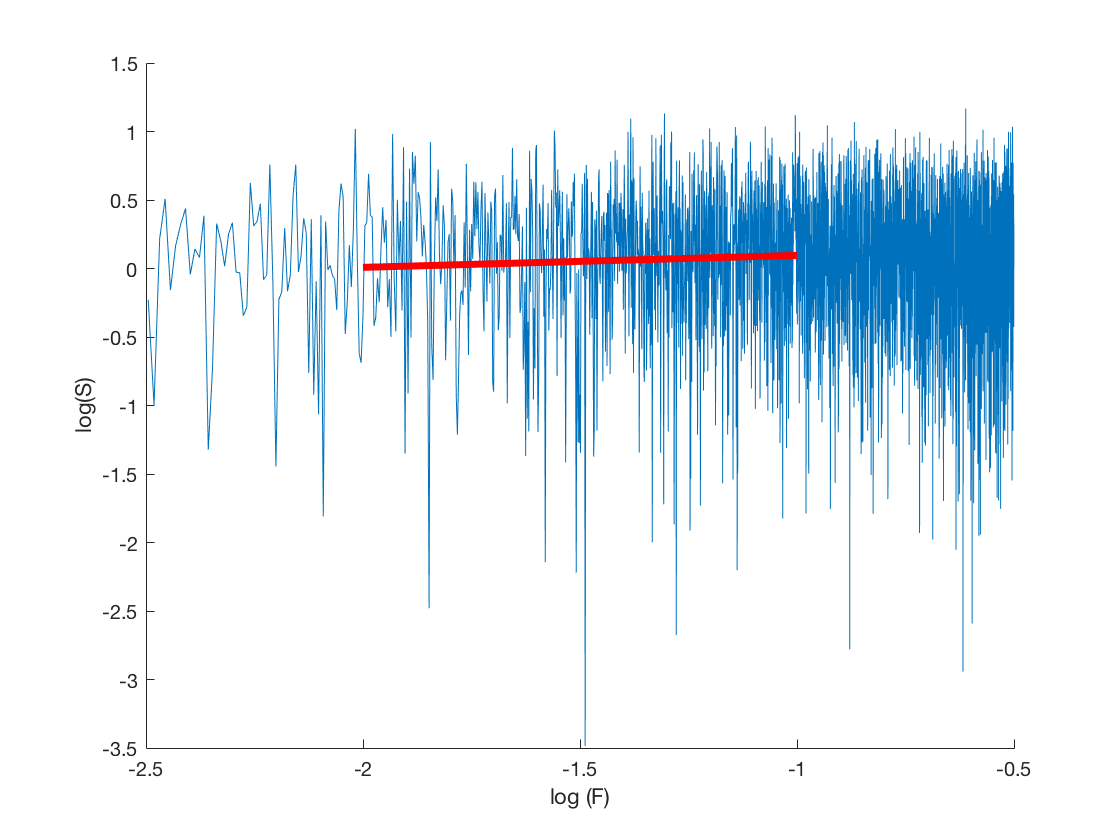
\includegraphics[width=0.8\linewidth]{figures/pseW.png}
		\end{figure}
		$\beta = -0.08$
	\end{column}
	
	\begin{column}{0.15\paperwidth}
		\vspace{2cm}\\
		$S(f)\sim f^{-\beta}$
		
	\end{column}
	
	\begin{column}{0.4\paperwidth}
		\centering
		Red
		
		\begin{figure}
			\centering
			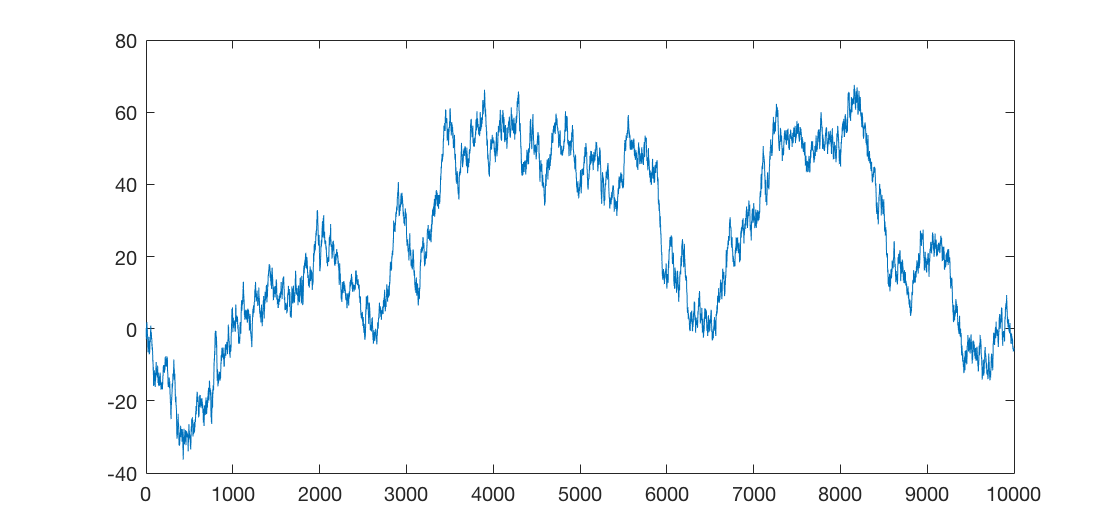
\includegraphics[width=0.8\linewidth]{figures/xr.png}
		\end{figure}
		\begin{figure}
			\centering
			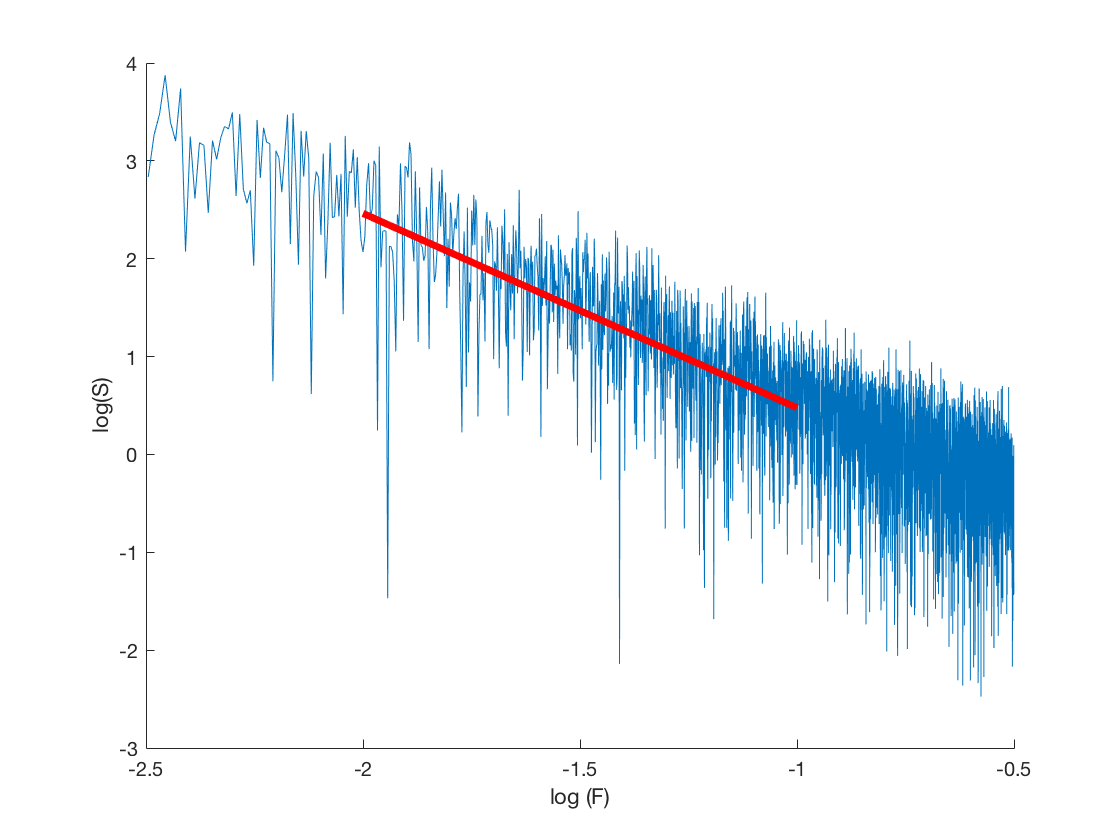
\includegraphics[width=0.8\linewidth]{figures/pseR.png}
		\end{figure}
		$\beta = 1.99$
	\end{column}
\end{columns}
\note{White noise has zero correlation, Brownian noise has ACF = 1. }
\end{frame}

\begin{frame}{But, be careful}
\begin{columns}
\begin{column}{0.4\paperwidth}
	\centering
	AR(1) model
	
	\begin{figure}
		\centering
		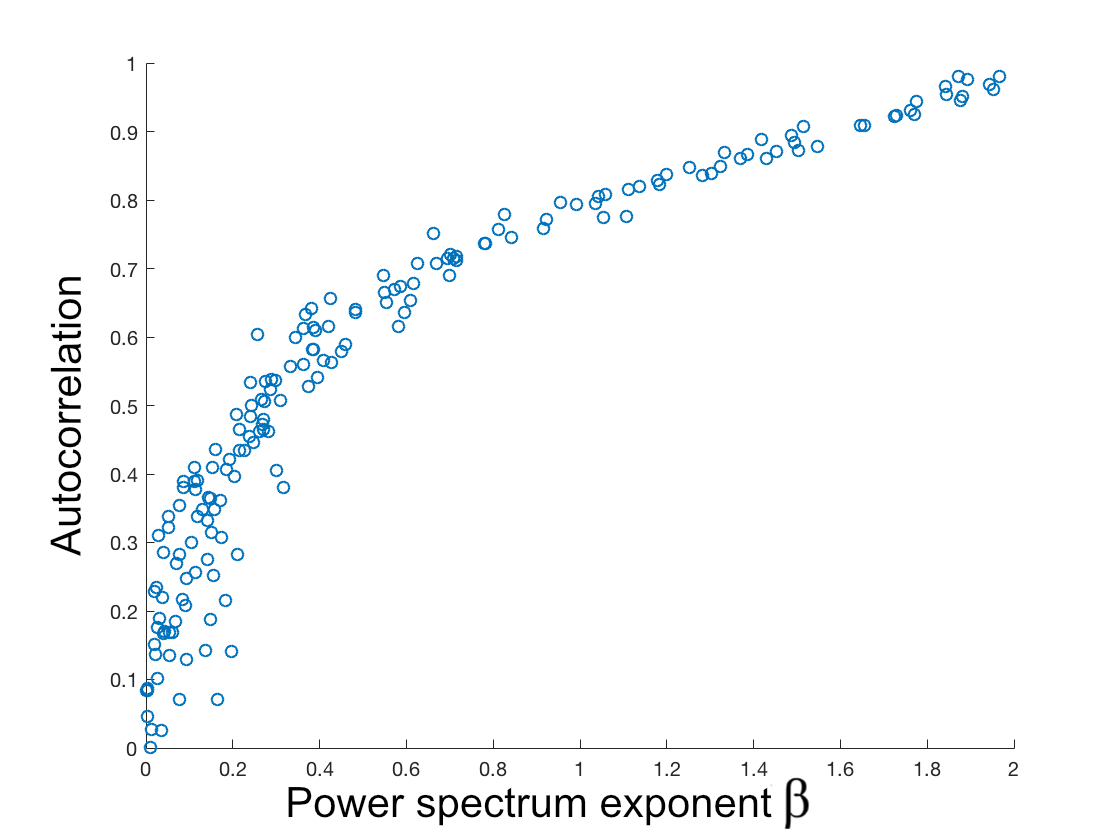
\includegraphics[width=0.9\linewidth]{figures/spectrum_armodel.png}
	\end{figure}
	
	$x_{n} = \phi x_{n-1} + \eta_{n}$\\
	\vfill
\end{column}

\begin{column}{0.4\paperwidth}
	\centering
	AR(63) model

	\begin{figure}
		\centering
		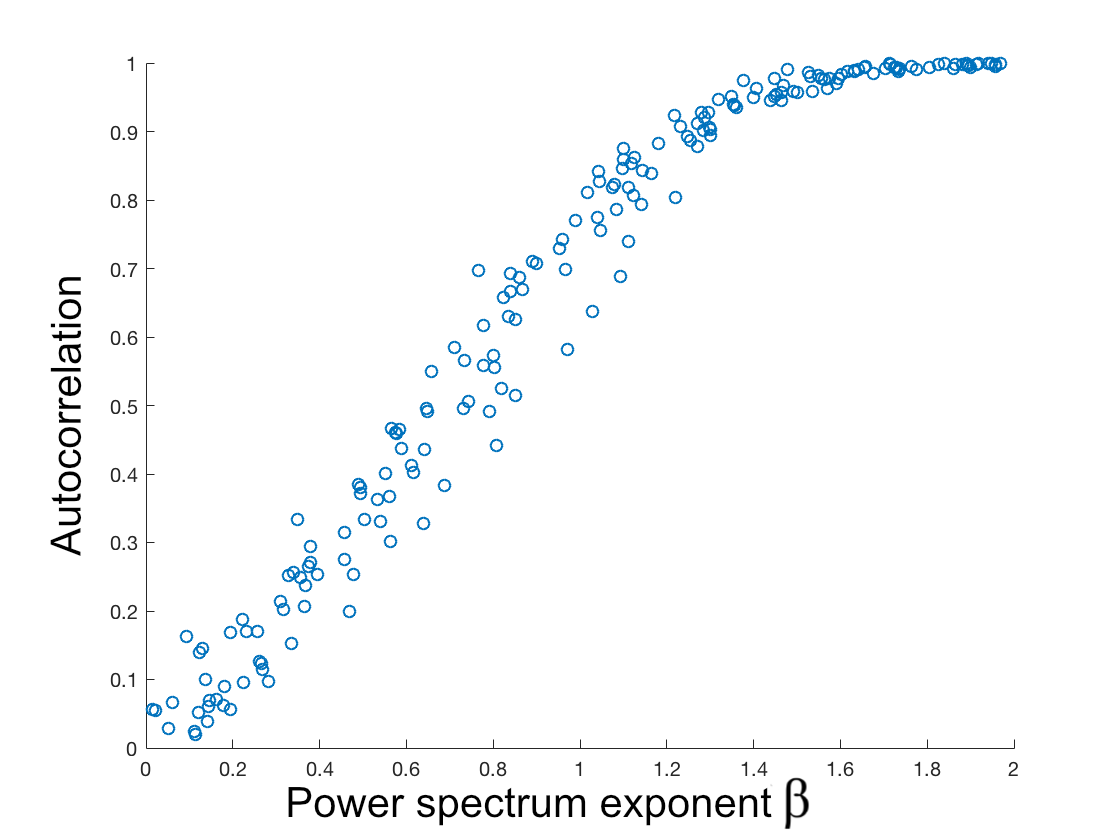
\includegraphics[width=0.9\linewidth]{figures/spectrum_noisegen.png}
	\end{figure}
	MatLab DSP Toolbox\\
	Kasdin, N.J. (1995)*\\
	\vfill
\end{column}
\end{columns}
\vspace{1cm}
{\scriptsize
*Kasdin, N.J. "Discrete Simulation of Colored Noise and Stochastic Processes and 1/f Power Law Noise Generation." Proceedings of the IEEE, Vol. 83, No. 5, 1995, pp. 802-827.}
\end{frame}



\begin{frame}{Comparison: pitchfork bifurcation}
\begin{columns}
	\begin{column}{0.4\paperwidth}
		Bifurcation occurs at t=600\\
		\vspace{1cm}
		PS-indicator definitely the worst

	\end{column}
	
	\begin{column}{0.5\paperwidth}
		
		\begin{figure}
			\centering
			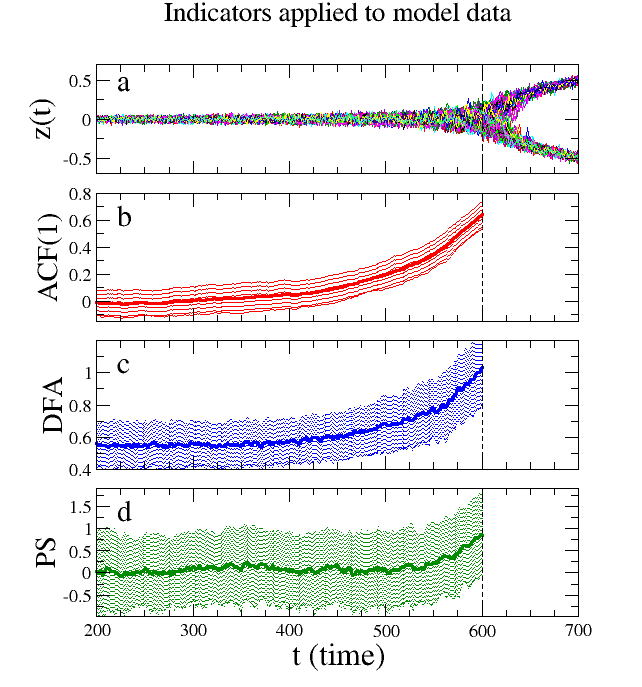
\includegraphics[width=\linewidth]{figures/Fig3_colour.png}
		\end{figure}

	\end{column}
\end{columns}

\end{frame}

\begin{frame}{Comparison: tropical cyclones}
\begin{columns}
	\begin{column}{0.4\paperwidth}
		Sea level pressure measurements taken at the landfall-location of 14 tropical cyclones.\\
		\vspace{1cm}
		PS-indicator works better than others\\
		\vspace{1cm}
		{\scriptsize Atlantic hurricanes Andrew (1992), Opal (1995), Floyd (1999), Charley (2004), Frances (2004), Jeanne (2004), Katrina (2005), Rita (2005), Ivan (2006) and Ernesto (2006); typhoons Zeb (1998), Megi (2010) and Flo (1990); and Cyclone Hudhud (2014)}
	\end{column}
	
	\begin{column}{0.5\paperwidth}
		
		\begin{figure}
			\centering
			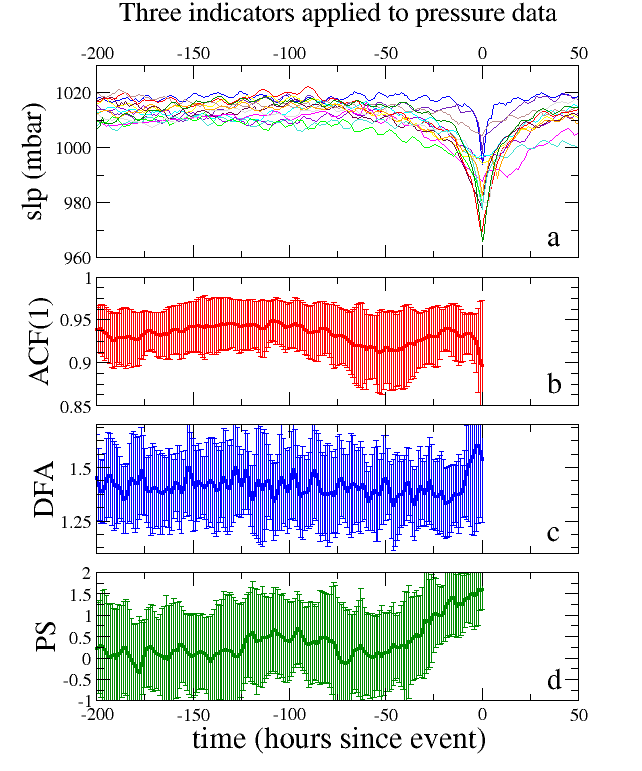
\includegraphics[width=\linewidth]{figures/fig4_colour.png}
		\end{figure}
		
	\end{column}
\end{columns}

\end{frame}


\begin{frame}{Thank you!}
Our paper: 
\begin{itemize}
	\footnotesize
	\item Prettyman, J., Kuna, T., Livina, V. (2018). A novel scaling indicator of early warning signals helps anticipate tropical cyclones. EPL (Europhysics Letters), 121(1), 10002.
\end{itemize}
\vspace{0.5cm}
Review of methods: 
\begin{itemize}
	\footnotesize
\item Livina, V. N., Ditlevsen, P. D., Lenton, T. M. (2012). An independent test of methods of detecting system states and bifurcations in time-series data. Physica A: Statistical Mechanics and its Applications, 391(3), 485-496.
\end{itemize}

\end{frame}

\begin{frame}{Two variables}
\begin{figure}
	\centering
	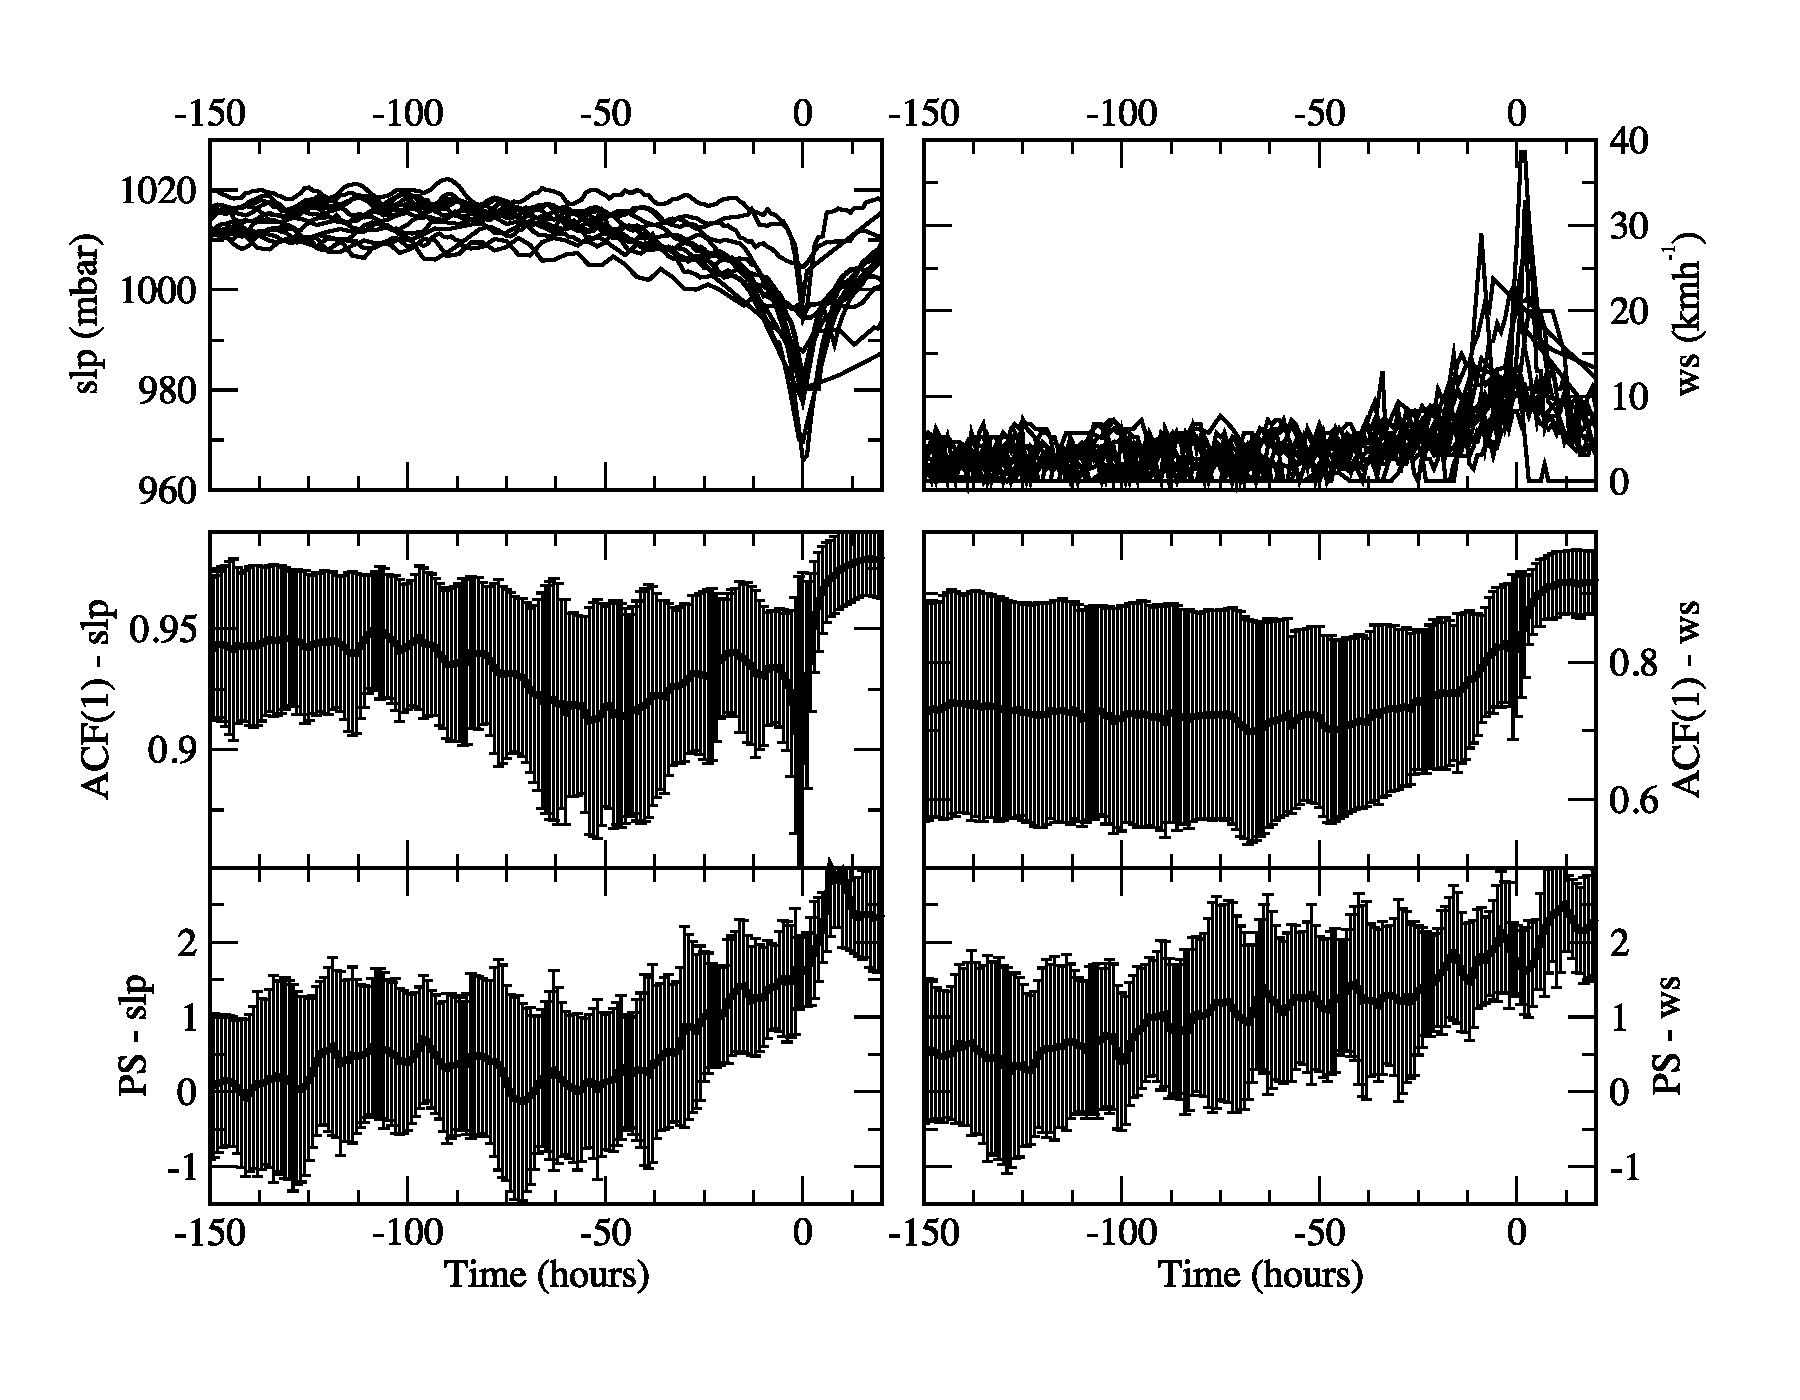
\includegraphics[width=0.9\linewidth]{figures/01_ACF1andPS.pdf}
\end{figure}
\end{frame}

\begin{frame}{Two variables: EOF method}
\begin{figure}
	\centering
	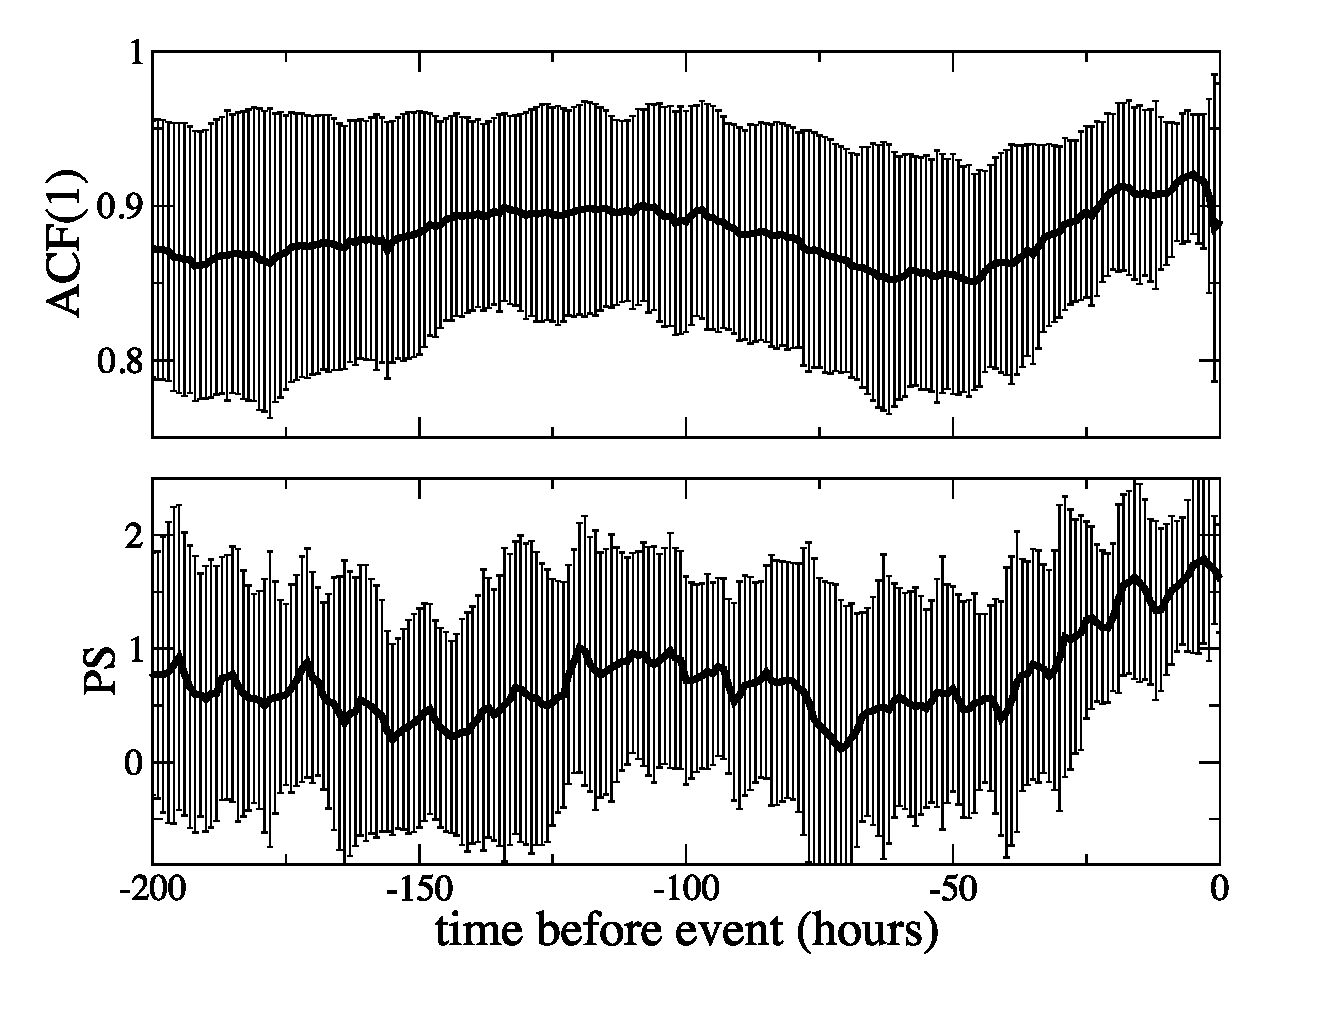
\includegraphics[width=0.7\linewidth]{figures/03_EOF.pdf}
\end{figure}
\end{frame}

\begin{frame}{Two variables: Williamson and Lenton method}
\begin{figure}
	\centering
	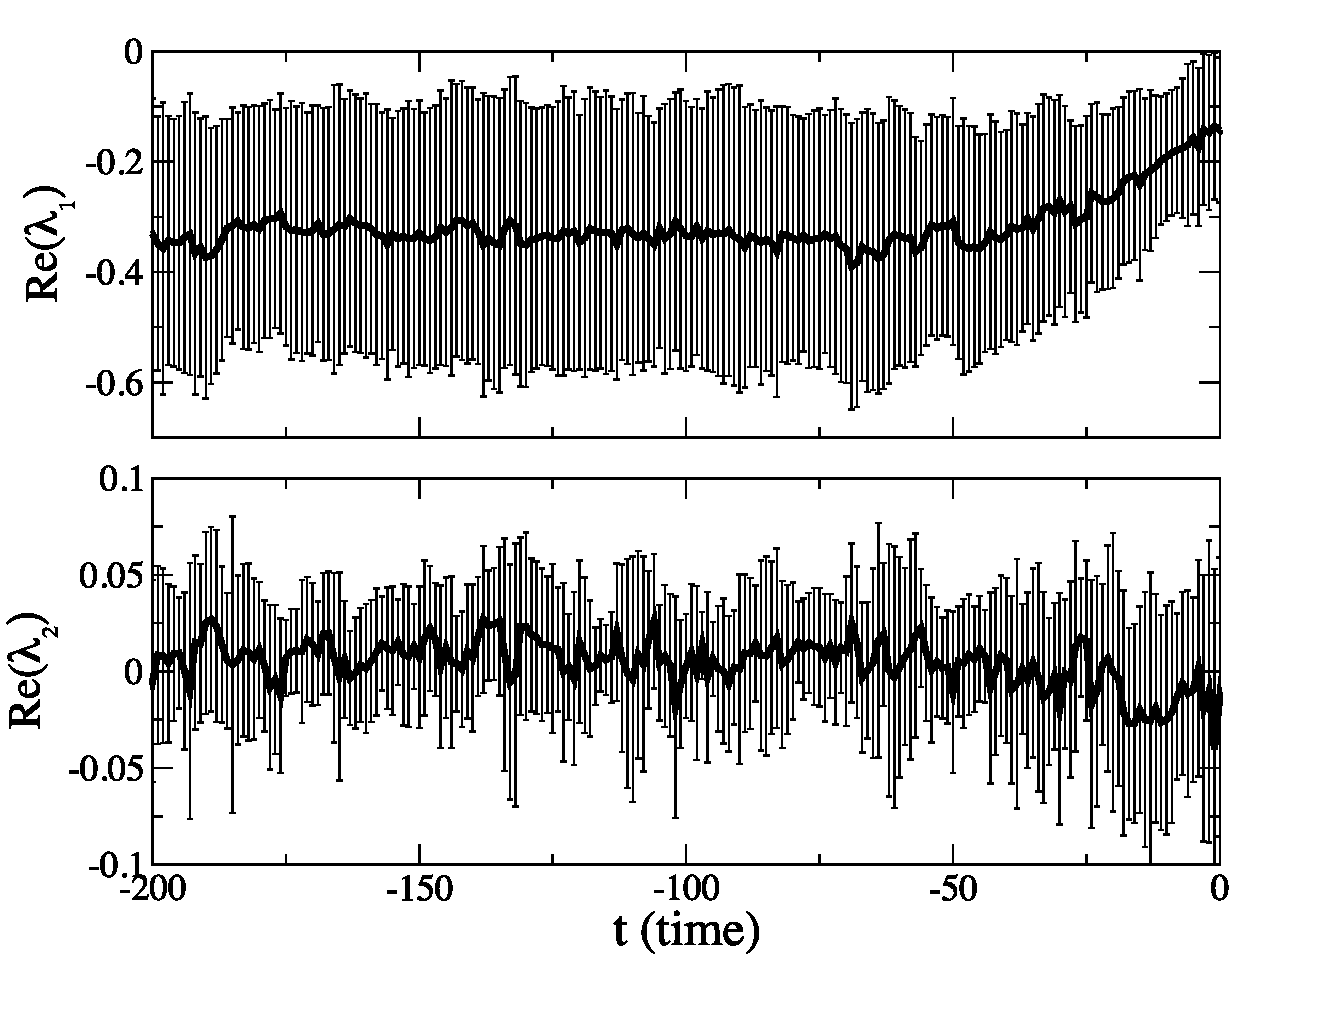
\includegraphics[width=0.7\linewidth]{figures/04_WL.pdf}
\end{figure}
{\scriptsize Williamson, M. S., Lenton, T. M. (2015). Detection of bifurcations in noisy coupled systems from multiple time series. Chaos: An Interdisciplinary Journal of Nonlinear Science, 25(3)}
\end{frame}

\end{document}











